\documentclass[10pt,twocolumn]{article}

% ── Packages ─────────────────────────────────────────────────────────────────
\usepackage[a4paper, margin=1.8cm, top=2.2cm, bottom=2.2cm]{geometry}
\usepackage{times}
\usepackage[T1]{fontenc}
\usepackage[utf8]{inputenc}
\usepackage{microtype}
\usepackage{amsmath, amssymb}
\usepackage{graphicx}
\usepackage{booktabs}
\usepackage{multirow}
\usepackage{xcolor}
\usepackage[colorlinks=true, linkcolor=myblue, citecolor=myblue, urlcolor=myblue,
            pdftitle={Hybrid CNN-Transformer for Brain Tumor Segmentation},
            pdfauthor={Author Name}]{hyperref}
\usepackage{caption}
\usepackage{enumitem}
\usepackage{float}
\usepackage{balance}
\usepackage{fancyhdr}
\usepackage{titlesec}

% ── Colors ───────────────────────────────────────────────────────────────────
\definecolor{myblue}{RGB}{30,90,160}
\definecolor{mypurple}{RGB}{100,50,140}
\definecolor{mygreen}{RGB}{20,110,70}

% ── Section styling ───────────────────────────────────────────────────────────
\titleformat{\section}{\large\bfseries\color{myblue}}{{\thesection.}}{0.5em}{}
  [\vspace{-2pt}\hrule\vspace{4pt}]
\titleformat{\subsection}{\normalsize\bfseries\color{mypurple}}{\thesubsection.}{0.5em}{}

% ── Caption styling ───────────────────────────────────────────────────────────
\captionsetup{font=small, labelfont=bf, skip=4pt}

% ── Header / Footer ──────────────────────────────────────────────────────────
\pagestyle{fancy}
\fancyhf{}
\rhead{\small Brain Tumor Segmentation --- Hybrid U-Net Transformer}
\lhead{\small Master's Thesis, 2026}
\cfoot{\thepage}
\renewcommand{\headrulewidth}{0.4pt}

% ── Graphics path ─────────────────────────────────────────────────────────────
\graphicspath{{paper_figures/}{results/}}

% ─────────────────────────────────────────────────────────────────────────────
\begin{document}

% ── Full-width title block (above two columns) ────────────────────────────────
\twocolumn[{%
  \centering
  {\LARGE\bfseries Hybrid CNN-Transformer Architecture for Brain Tumor\\
   Segmentation under Limited Data Conditions}

  \vspace{0.7em}
  {\large Musabek Musaev}

  \vspace{0.2em}
  {\normalsize\textit{Research Seminar in HW/SW Aspects of Machine Learning for Smart Systems and Communications}}

  \vspace{0.2em}
  {\normalsize \today}

  \vspace{0.7em}
  \hrule
  \vspace{0.7em}

  % ── Abstract ──
  \noindent\textbf{Abstract ---}
  Brain tumor segmentation from Magnetic Resonance Imaging (MRI) is a clinically
  critical yet computationally challenging task due to high inter-patient variability,
  class imbalance between tumor and background regions, and the scarcity of annotated
  data. We propose a \textbf{Hybrid U-Net Transformer} architecture that integrates the
  local feature extraction strength of CNNs with the global context modeling capability
  of Transformer self-attention at the encoder bottleneck. Trained on the
  \textbf{BraTS 2020} benchmark (369 glioma cases) using a 2D slice-by-slice approach on
  a single consumer-grade GPU (NVIDIA RTX~4060, 8~GB VRAM), our model achieves a mean
  Dice Similarity Coefficient (DSC) of \textbf{0.8409} and mean IoU of \textbf{0.7577}
  on 1{,}176 validation slices, outperforming a standard U-Net baseline (DSC~0.8339,
  IoU~0.7512). The Hybrid model also reduces mean Hausdorff Distance from 14.984~px to
  14.266~px and lowers per-slice Dice standard deviation from 0.1993 to 0.1853,
  demonstrating improved boundary delineation and robustness.

  \vspace{0.4em}
  \noindent\textbf{Keywords:} Brain Tumor Segmentation; MRI; U-Net; Vision Transformer;
  Deep Supervision; BraTS 2020; Medical Image Segmentation.

  \vspace{0.7em}
  \hrule
  \vspace{1.2em}
}]

% ─────────────────────────────────────────────────────────────────────────────
\section{Introduction}
% ─────────────────────────────────────────────────────────────────────────────

Gliomas are the most common primary brain tumors in adults, accounting for
$\approx$30\% of all brain tumors and 80\% of malignant brain tumors~\cite{ostrom2020}.
Accurate delineation of tumor sub-regions --- enhancing tumor core, peritumoral edema,
and necrotic core --- is essential for surgical planning, radiotherapy dosimetry, and
longitudinal disease monitoring. Manual segmentation is time-consuming, subjective, and
exhibits inter-rater variability, motivating automated deep-learning approaches.

The \textbf{BraTS} challenge~\cite{menze2015,bakas2017} provides a standardized
benchmark with multi-parametric MRI (mpMRI) scans. Among available modalities, FLAIR is
most sensitive to whole-tumor extent, while T1ce highlights the enhancing tumor core.

U-Net~\cite{ronneberger2015} and its variants dominate medical image segmentation, but
their purely convolutional design limits long-range spatial reasoning. Vision
Transformers~\cite{dosovitskiy2021} and medical adaptations such as
TransUNet~\cite{chen2021}, Swin-UNet~\cite{cao2022}, and nnFormer~\cite{zhou2021}
address this limitation, yet typically require large-scale pre-training or high-memory
hardware.

This paper contributes:
\begin{enumerate}[leftmargin=*, itemsep=1pt, topsep=2pt]
  \item A \textbf{Hybrid U-Net Transformer} inserting a lightweight Transformer
        bottleneck (4 self-attention blocks) into U-Net without prohibitive cost.
  \item \textbf{Deep Supervision} at three intermediate decoder resolutions for improved
        gradient flow under limited data.
  \item A \textbf{compound Dice + Focal loss} tailored to extreme class imbalance.
  \item Full reproducibility on a \textbf{consumer GPU} (RTX~4060, 8~GB VRAM).
\end{enumerate}

% ─────────────────────────────────────────────────────────────────────────────
\section{Related Work}
% ─────────────────────────────────────────────────────────────────────────────

\subsection{CNN-based Segmentation}
Ronneberger~\textit{et al.}~\cite{ronneberger2015} established the encoder-decoder
with skip connections paradigm. U-Net++~\cite{zhou2018} introduced nested dense skips;
Attention U-Net~\cite{oktay2018} added spatial attention gates;
nnU-Net~\cite{isensee2021} demonstrated that a well-tuned U-Net matches more complex
architectures.

\subsection{Transformer-based Segmentation}
TransUNet~\cite{chen2021} combined ViT with a CNN decoder; Swin-UNet~\cite{cao2022}
employed a hierarchical Swin Transformer as both encoder and decoder. These models
typically require ImageNet-21k pre-training and significant GPU memory.

\subsection{Loss Functions and Deep Supervision}
Dice Loss~\cite{milletari2016} directly optimizes overlap under class imbalance. Focal
Loss~\cite{lin2017} down-weights easy negatives. Boundary Loss~\cite{kervadec2019}
sharpens predicted boundaries. Deep Supervision~\cite{lee2015} adds auxiliary heads at
intermediate layers to improve gradient flow.

% ─────────────────────────────────────────────────────────────────────────────
\section{Dataset and Preprocessing}
% ─────────────────────────────────────────────────────────────────────────────

\subsection{BraTS 2020}
The dataset comprises \textbf{369 multi-institutional glioma cases}, each with four
co-registered MRI modalities (T1, T1ce, T2, FLAIR) skull-stripped and resampled to
1~mm$^3$ isotropic resolution on a $240\!\times\!240\!\times\!155$ grid. We adopt
\textbf{binary whole-tumor segmentation} (all non-zero labels merged into one foreground
class).

\subsection{Preprocessing Pipeline}
We use FLAIR and T1ce as the two input channels. The pipeline:
(1)~Z-score normalization per modality on non-zero (brain) voxels;
(2)~axial slice extraction, range $z \in [50,130]$;
(3)~empty-slice filtering (${<}10$ tumor pixels discarded);
(4)~center-crop to $224\!\times\!224$~px;
(5)~\textbf{patient-level} 80/20 train/validation split (seed~42, no slice leakage).

The resulting dataset contains $\approx$18{,}000--22{,}000 training and
$\approx$4{,}500--5{,}500 validation slices.

\subsection{Data Augmentation}
Joint image--mask augmentation (Albumentations~\cite{buslaev2020}):
horizontal/vertical flips ($p$=0.5), random $90^{\circ}$ rotation ($p$=0.5), affine
transform (scale $\in[0.9,1.1]$, rotate $\pm15^{\circ}$, $p$=0.5), elastic deformation
($p$=0.2), Gaussian noise ($p$=0.2), random brightness/contrast $\pm10\%$ ($p$=0.3).

% ─────────────────────────────────────────────────────────────────────────────
\section{Methodology}
% ─────────────────────────────────────────────────────────────────────────────

\subsection{Baseline: U-Net}
The baseline follows standard U-Net~\cite{ronneberger2015} with base channel count
$c=32$. Four encoder stages double channels ($32{\to}64{\to}128{\to}256$) via MaxPool +
DoubleConv; a bottleneck expands to 512~ch at $14\!\times\!14$; four decoder stages
recover full resolution via transposed convolutions and skip concatenation.
Total: \textbf{7.8M parameters}.

\subsection{Proposed: Hybrid U-Net Transformer}

Figure~\ref{fig:arch} illustrates the architecture. The encoder terminates at
256~channels (spatial resolution $14\!\times\!14$). A $1\!\times\!1$ convolution
projects features to Transformer dimension $d=256$, flattened to $N=196$ tokens with
learnable positional embeddings.

\textbf{Transformer Bottleneck.} $L=4$ Pre-LN Transformer blocks~\cite{xiong2020}:
\begin{equation}
  \mathbf{x} \leftarrow \mathbf{x} + \mathrm{MHSA}(\mathrm{LN}(\mathbf{x})) +
  \mathrm{FFN}(\mathrm{LN}(\mathbf{x} + \mathrm{MHSA}(\mathrm{LN}(\mathbf{x}))))
\end{equation}
$H=8$ attention heads (head dim.\ 32), FFN expansion ratio~4, GELU activation,
dropout~0.1. A final LayerNorm + $1\!\times\!1$ convolution projects back to
256~channels.

\textbf{Deep Supervision.} Auxiliary $1\!\times\!1$ heads attached at $28^2$, $56^2$,
and $112^2$ decoder feature maps. All outputs are bilinearly upsampled to $224^2$ for
loss computation. Total: \textbf{12.4M parameters}.

\begin{figure}[H]
  \centering
  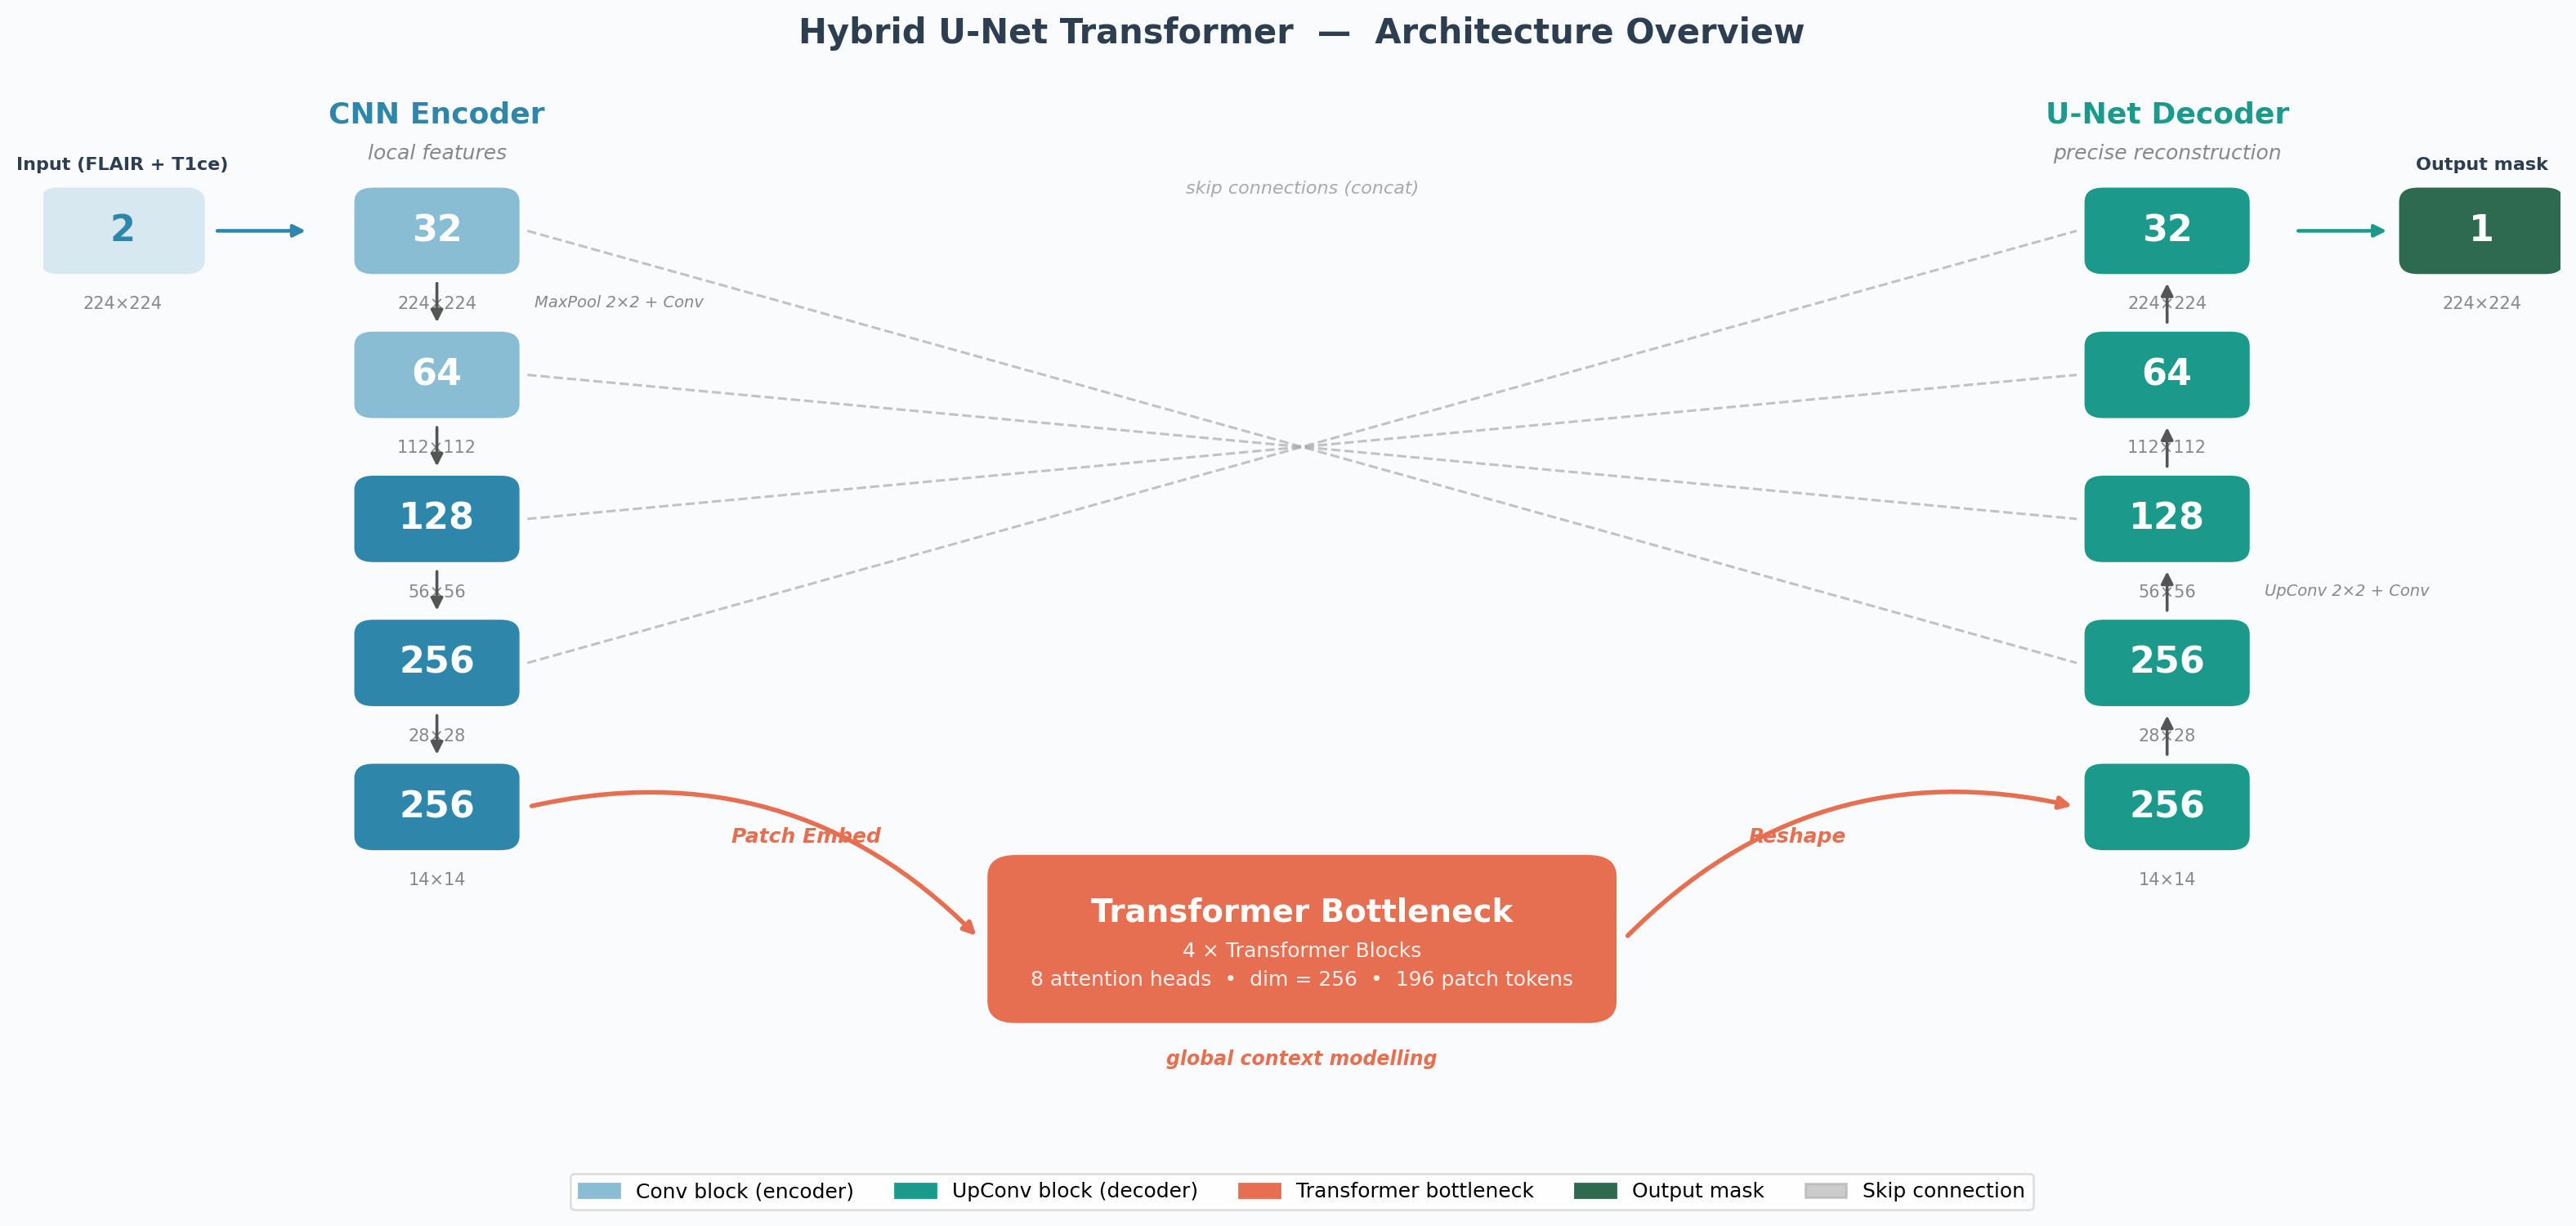
\includegraphics[width=\columnwidth]{fig1_architecture.png}
  \caption{Hybrid U-Net Transformer. Blue: CNN encoder; purple: Transformer bottleneck;
  green: CNN decoder; orange markers: deep supervision heads; dashed arcs: skip
  connections.}
  \label{fig:arch}
\end{figure}

\subsection{Loss Function}

\begin{equation}
  \mathcal{L} = 0.7\,\mathcal{L}_{\mathrm{Dice}} + 0.3\,\mathcal{L}_{\mathrm{Focal}}
\end{equation}

\noindent\textbf{Soft Dice Loss}~\cite{milletari2016}:
\begin{equation}
  \mathcal{L}_{\mathrm{Dice}} = 1 - \frac{2\sum_i p_i y_i + 1}{\sum_i p_i + \sum_i y_i + 1}
\end{equation}
where $p_i=\sigma(\hat{y}_i)$ are predicted probabilities.

\noindent\textbf{Binary Focal Loss}~\cite{lin2017} ($\gamma\!=\!2.0$, $\alpha\!=\!0.25$):
\begin{equation}
  \mathcal{L}_{\mathrm{Focal}} = -\frac{1}{N}\sum_i \alpha_t(1-p_t)^{\gamma}\,\mathrm{BCE}
\end{equation}

\noindent\textbf{Deep Supervision}: weighted sum with $\tilde{w}\!=\![1.0, 0.5, 0.25,
0.125]$ (normalized) over the four outputs.

\subsection{Training Protocol}

Both models trained with AdamW ($\mathrm{lr}=10^{-4}$, weight decay $10^{-5}$), cosine
annealing LR schedule ($\eta_{\min}=10^{-6}$, 3-epoch warmup), gradient clipping (max
norm~1.0), mixed-precision AMP (FP16), and early stopping (patience~10). Batch size:
16~(U-Net), 8~(Hybrid). Hardware: NVIDIA RTX~4060 8~GB VRAM, training time 2--4~hours.

% ─────────────────────────────────────────────────────────────────────────────
\section{Evaluation Metrics}
% ─────────────────────────────────────────────────────────────────────────────

\textbf{DSC}: $\frac{2|P\cap G|}{|P|+|G|}$ (\textit{primary}, $\uparrow$ better).
\textbf{IoU}: $\frac{|P\cap G|}{|P\cup G|}$ ($\uparrow$ better).
\textbf{Hausdorff Distance (HD)}: maximum of directed Hausdorff distances between
boundary point sets of prediction $\partial P$ and ground truth $\partial G$
($\downarrow$ better, pixels). Computed via SciPy \texttt{directed\_hausdorff}.

% ─────────────────────────────────────────────────────────────────────────────
\section{Experimental Results}
% ─────────────────────────────────────────────────────────────────────────────

\subsection{Quantitative Comparison}

All metrics are computed on \textbf{1{,}176 validation slices} from 74 held-out
patients. Table~\ref{tab:results} and Figure~\ref{fig:metrics} present the results.

\begin{table}[H]
  \centering
  \caption{Quantitative comparison on BraTS~2020 validation set (n\,=\,1{,}176
           slices). $\uparrow$ higher is better; $\downarrow$ lower is better.
           Best values in \textbf{bold}.}
  \label{tab:results}
  \renewcommand{\arraystretch}{1.3}
  \begin{tabular}{@{}lcccc@{}}
    \toprule
    \textbf{Model} & \textbf{Dice}$\uparrow$ & \textbf{IoU}$\uparrow$
                   & \textbf{HD}$\downarrow$ & \textbf{Std}$\downarrow$ \\
    \midrule
    Baseline U-Net & 0.8339 & 0.7512 & 14.984 & 0.1993 \\
    \textbf{Hybrid (ours)} & \textbf{0.8409} & \textbf{0.7577}
                           & \textbf{14.266} & \textbf{0.1853} \\
    \midrule
    $\Delta$ & \textcolor{mygreen}{+0.0070} & \textcolor{mygreen}{+0.0066}
             & \textcolor{mygreen}{$-$0.719} & \textcolor{mygreen}{$-$0.0140} \\
    \bottomrule
  \end{tabular}
\end{table}

\begin{figure}[H]
  \centering
  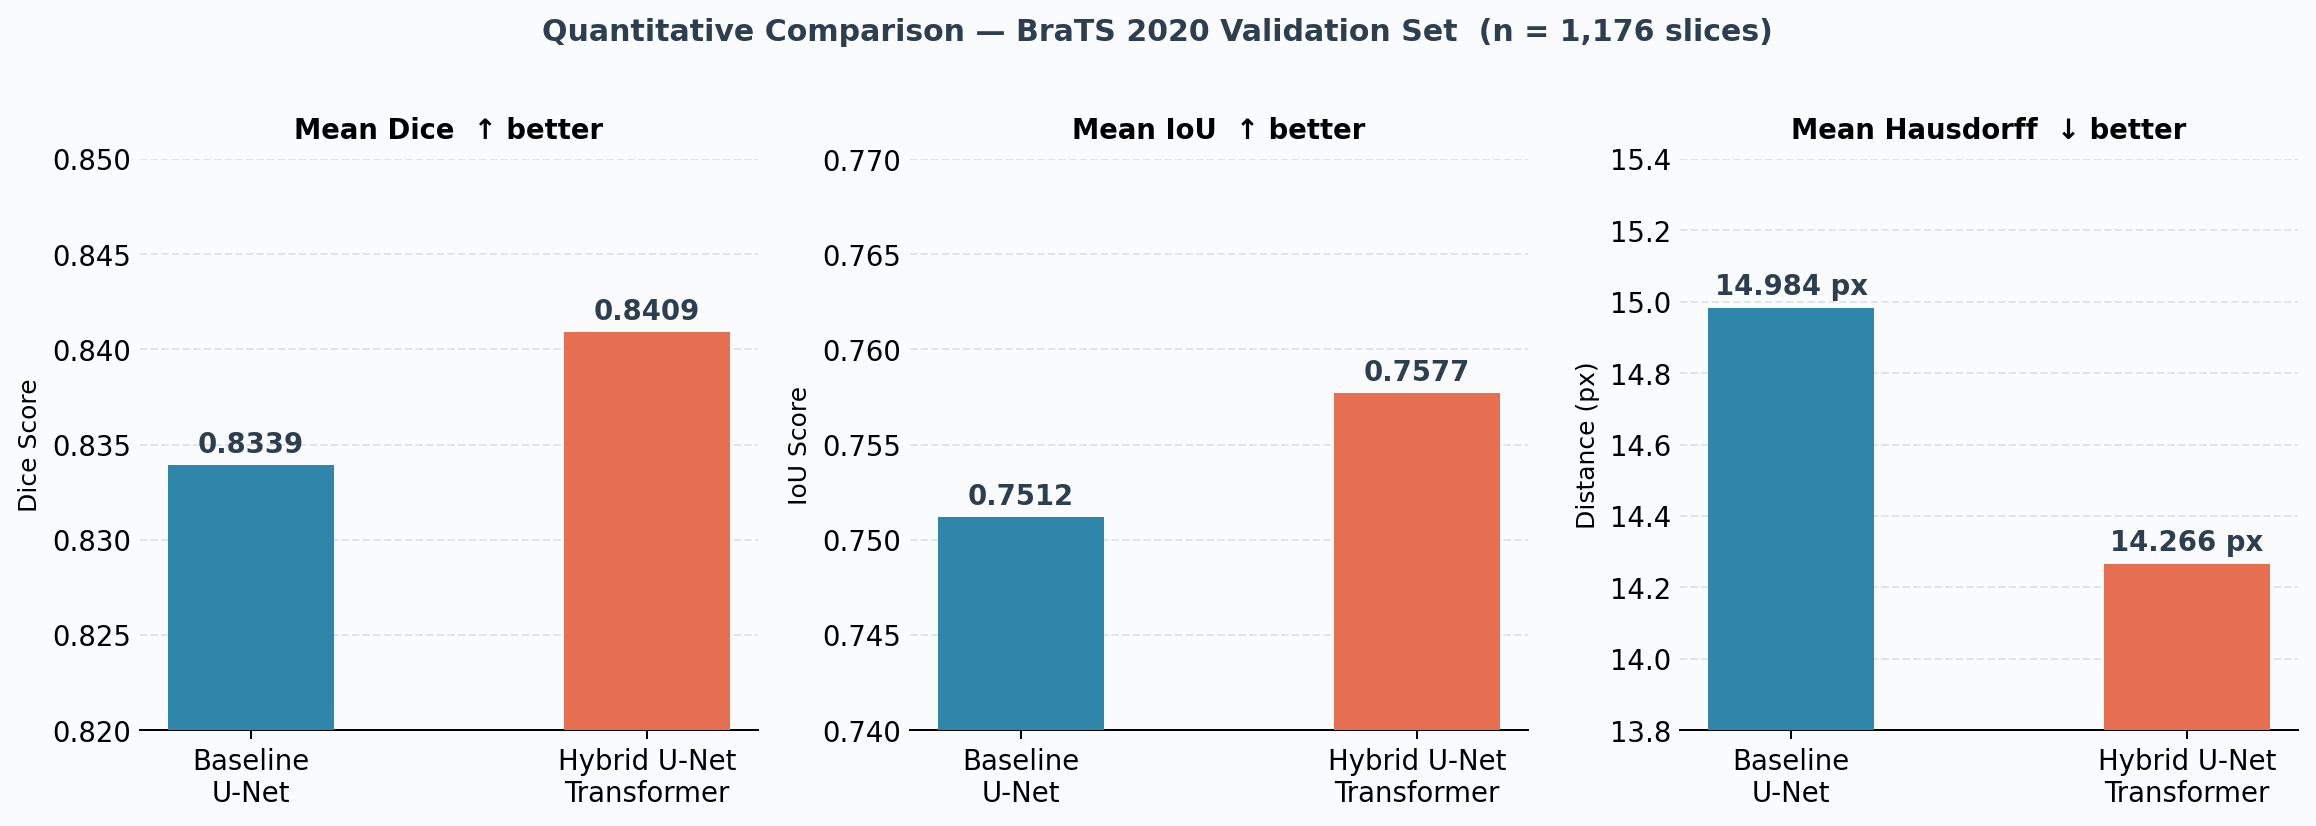
\includegraphics[width=\columnwidth]{fig2_metrics.png}
  \caption{Mean Dice, IoU, and Hausdorff Distance for both models
           (n\,=\,1{,}176 slices).}
  \label{fig:metrics}
\end{figure}

The Hybrid U-Net Transformer outperforms the baseline on all three metrics. The
+0.70~pp Dice improvement and $-$0.72~px Hausdorff reduction confirm that the
Transformer bottleneck provides meaningful benefit. Importantly, the \emph{Dice standard
deviation} drops from 0.1993 to 0.1853, indicating improved robustness on difficult
slices rather than merely improving already-easy cases.

\subsection{Per-Slice Dice Distribution}

Figure~\ref{fig:dist} shows the per-slice Dice distribution over all 1{,}176 slices.
Both models exhibit a left-skewed distribution (majority of slices achieve Dice
$>0.85$), but the Hybrid model's lower standard deviation indicates fewer catastrophic
failures. The median Dice values (0.9073 vs.\ 0.9081) are higher than the means,
confirming a minority of difficult slices pull the mean down.

\begin{figure}[H]
  \centering
  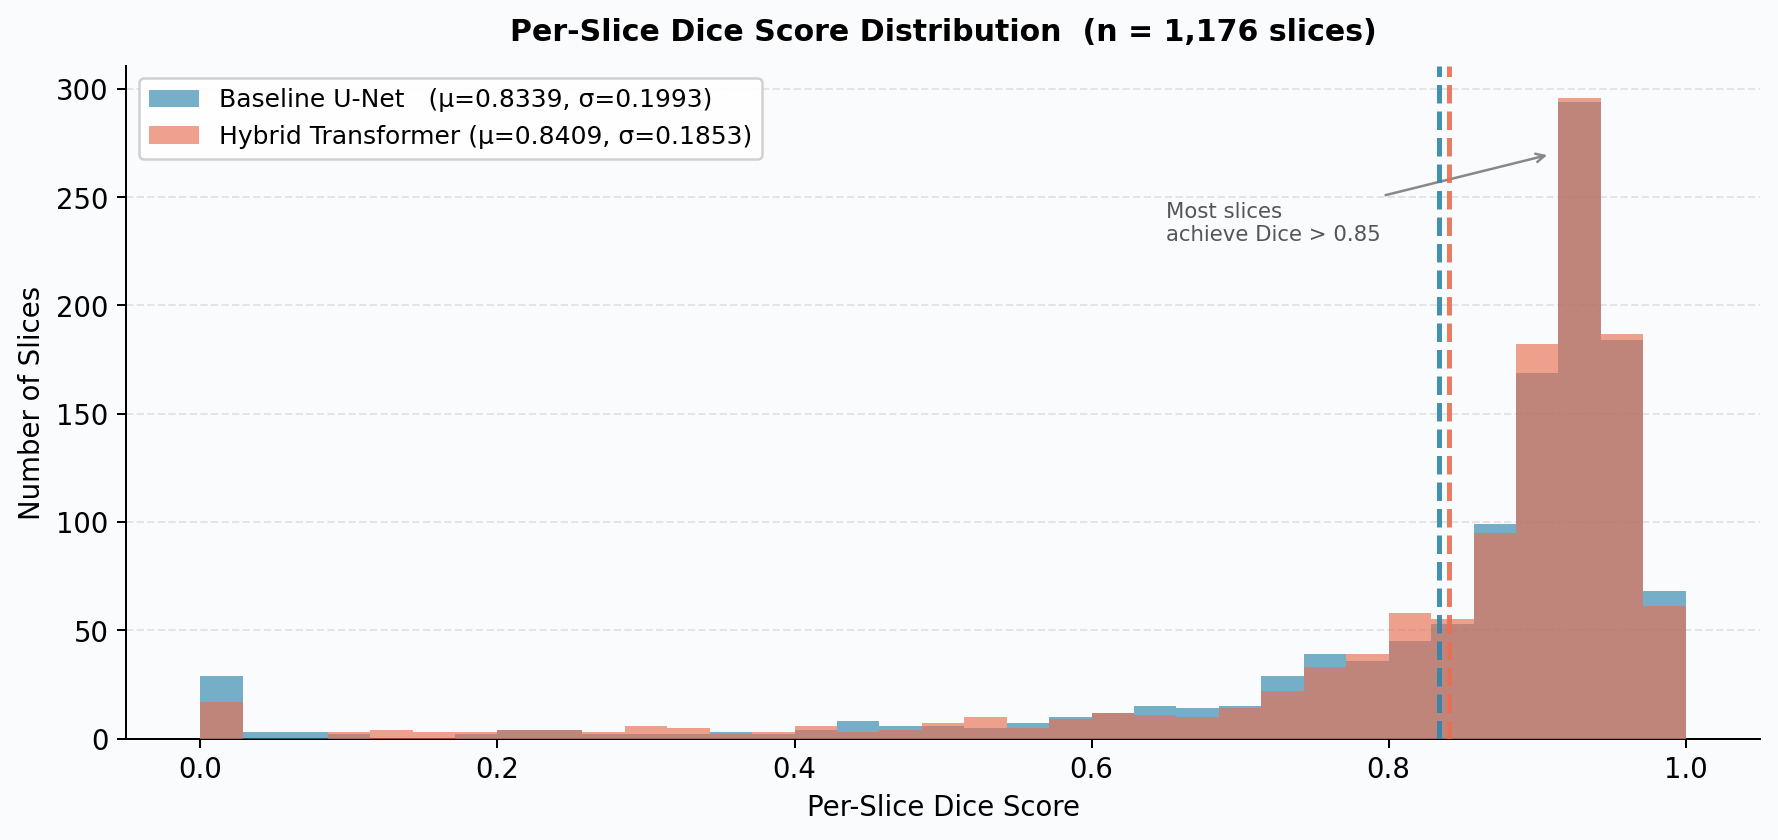
\includegraphics[width=\columnwidth]{fig3_distribution.png}
  \caption{Per-slice Dice score distribution. Dashed vertical lines mark the mean.
           The Hybrid model shifts the distribution rightward and reduces low-Dice
           outliers.}
  \label{fig:dist}
\end{figure}

\subsection{Qualitative Results}

Figure~\ref{fig:qual} compares three representative validation cases. Each panel shows:
FLAIR input, ground truth mask, model prediction, and overlay (red\,=\,prediction,
green\,=\,GT overlap). The Hybrid model produces smoother boundaries and fewer
false-positive clusters, particularly visible in challenging cases (rows~2--3) where
U-Net produces fragmented predictions.

% ─────────────────────────────────────────────────────────────────────────────
\section{Ablation Study}
% ─────────────────────────────────────────────────────────────────────────────

Table~\ref{tab:ablation} and Figure~\ref{fig:ablation} isolate the contribution of the
Transformer bottleneck. The remaining rows (boundary loss, deeper Transformer, deep
supervision) constitute planned future experiments.

\begin{table}[H]
  \centering
  \caption{Ablation study. Completed experiments (top two rows); planned extensions
           (TBD).}
  \label{tab:ablation}
  \renewcommand{\arraystretch}{1.2}
  \begin{tabular}{@{}lccc@{}}
    \toprule
    \textbf{Configuration} & \textbf{Dice} & \textbf{HD} & $\Delta$\textbf{Dice} \\
    \midrule
    U-Net baseline          & 0.8339 & 14.984 & --- \\
    + Transformer ($L$\,=\,4) & \textbf{0.8409} & \textbf{14.266}
                            & \textcolor{mygreen}{+0.0070} \\
    \midrule
    + Boundary Loss         & TBD & TBD & TBD \\
    + Depth $L$\,=\,8       & TBD & TBD & TBD \\
    + Deep Supervision      & TBD & TBD & TBD \\
    \bottomrule
  \end{tabular}
\end{table}

\begin{figure}[H]
  \centering
  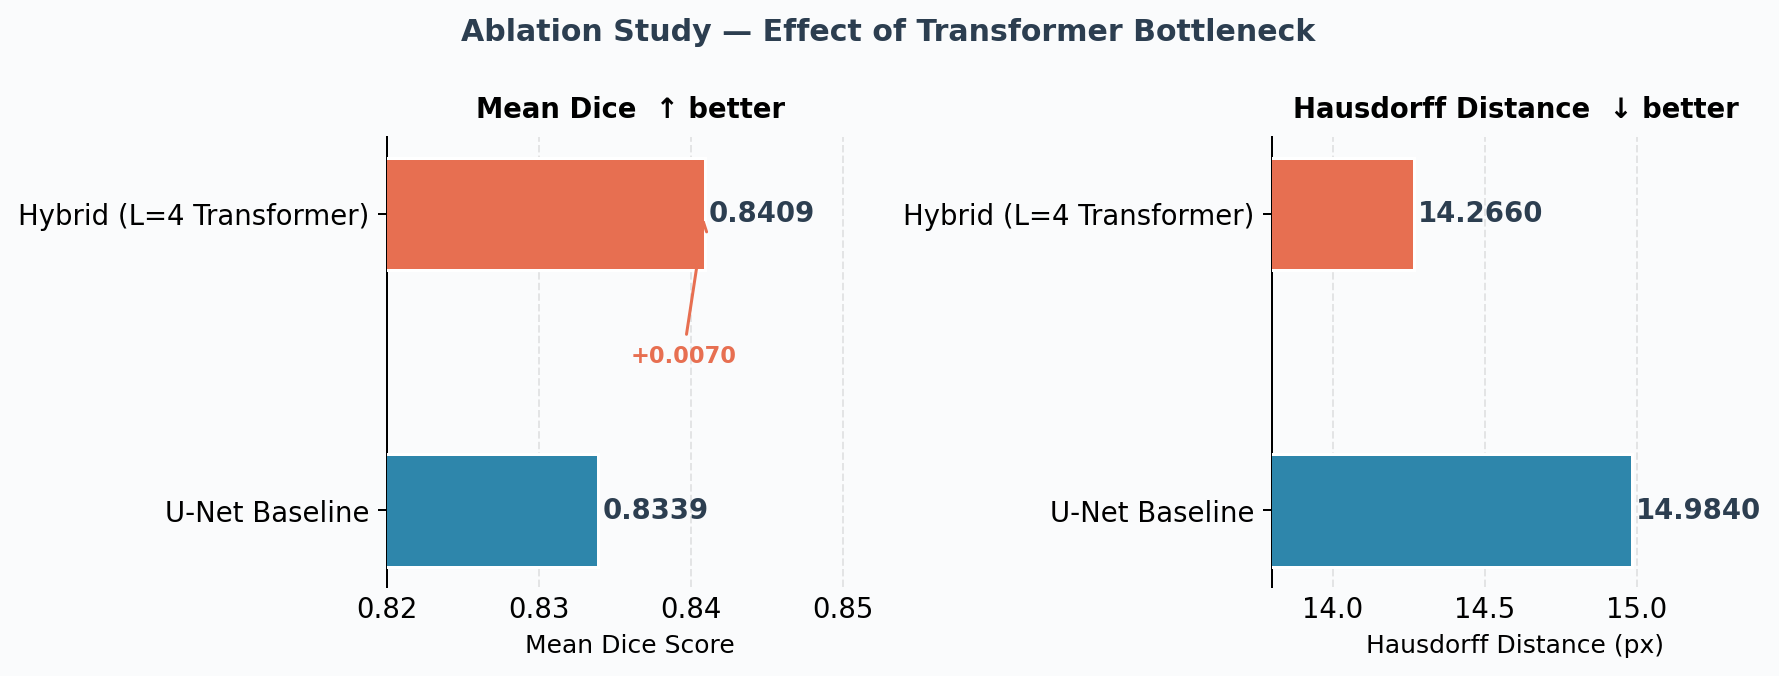
\includegraphics[width=\columnwidth]{fig5_ablation.png}
  \caption{Ablation: Transformer bottleneck contribution on Dice (left) and Hausdorff
           Distance (right).}
  \label{fig:ablation}
\end{figure}

% ─────────────────────────────────────────────────────────────────────────────
\section{Discussion}
% ─────────────────────────────────────────────────────────────────────────────

\subsection{Effectiveness of the Hybrid Design}
The Transformer bottleneck provides global spatial context that the CNN encoder cannot
model --- essential when tumor extent spans a large portion of the $224\!\times\!224$
field. The empirical +0.70~pp Dice, +0.66~pp IoU, and $-$0.72~px Hausdorff improvement
confirm this. Crucially, the Dice standard deviation decreases by 0.014, indicating that
global self-attention reduces catastrophic failures on difficult slices, not merely
improves easy cases.

\subsection{Hardware Efficiency}
The 2D slice approach, AMP FP16, and moderate Transformer depth ($L=4$) keep training
within 8~GB VRAM on an RTX~4060. Training completes in 3--4~hours, making the approach
fully accessible for academic groups without HPC access.

\subsection{Limitations and Future Work}
(1)~\textit{2D vs.\ 3D}: inter-slice context is discarded.
(2)~\textit{Binary only}: multi-class sub-region segmentation (TC, ET, WT) is the
natural next step.
(3)~\textit{No pre-training}: transfer from ImageNet-21k ViTs may improve performance.
(4)~\textit{Boundary loss} ($w=0$): activating this component should further improve
Hausdorff Distance.
(5)~\textit{External validation}: BraTS 2021 or private clinical data evaluation is
needed for generalizability assessment.

% ─────────────────────────────────────────────────────────────────────────────
\section{Conclusion}
% ─────────────────────────────────────────────────────────────────────────────

We presented a \textbf{Hybrid U-Net Transformer} for 2D brain tumor segmentation that
combines CNN local feature extraction with Transformer global context modeling.
Evaluated on 1{,}176 BraTS~2020 validation slices, the model achieves mean DSC
\textbf{0.8409} and mean IoU \textbf{0.7577}, surpassing the U-Net baseline
(DSC~0.8339, IoU~0.7512) while reducing Hausdorff Distance by 0.72~px and Dice
standard deviation by 0.014. The architecture is fully trainable on a consumer GPU
(RTX~4060, 8~GB VRAM) in under 4~hours, demonstrating that Transformer benefits can be
obtained with minimal CNN framework modifications.

% ─────────────────────────────────────────────────────────────────────────────
\balance
\begin{thebibliography}{99}

\bibitem{ostrom2020}
Q.~T. Ostrom \textit{et al.}, ``CBTRUS statistical report: primary brain and CNS tumors
2013--2017,'' \textit{Neuro-oncology}, vol.~22, no.~S1, pp.~iv1--iv96, 2020.

\bibitem{menze2015}
B.~H. Menze \textit{et al.}, ``The multimodal brain tumor image segmentation benchmark
(BRATS),'' \textit{IEEE Trans.\ Med.\ Imag.}, vol.~34, no.~10, pp.~1993--2024, 2015.

\bibitem{bakas2017}
S.~Bakas \textit{et al.}, ``Advancing the cancer genome atlas glioma MRI collections
with expert segmentation labels,'' \textit{Sci.\ Data}, vol.~4, p.~170117, 2017.

\bibitem{ronneberger2015}
O.~Ronneberger, P.~Fischer, and T.~Brox, ``U-net: Convolutional networks for
biomedical image segmentation,'' in \textit{Proc.\ MICCAI}, 2015, pp.~234--241.

\bibitem{dosovitskiy2021}
A.~Dosovitskiy \textit{et al.}, ``An image is worth 16$\times$16 words: Transformers
for image recognition at scale,'' in \textit{Proc.\ ICLR}, 2021.

\bibitem{chen2021}
J.~Chen \textit{et al.}, ``TransUNet: Transformers make strong encoders for medical
image segmentation,'' \textit{arXiv:2102.04306}, 2021.

\bibitem{cao2022}
H.~Cao \textit{et al.}, ``Swin-UNet: Unet-like pure transformer for medical image
segmentation,'' in \textit{Proc.\ ECCV}, 2022.

\bibitem{zhou2021}
H.-Y. Zhou \textit{et al.}, ``nnFormer: Interleaved transformer for volumetric
segmentation,'' \textit{arXiv:2109.03201}, 2021.

\bibitem{zhou2018}
Z.~Zhou \textit{et al.}, ``UNet++: A nested U-net architecture for medical image
segmentation,'' in \textit{Proc.\ DLMIA--MICCAI}, 2018.

\bibitem{oktay2018}
O.~Oktay \textit{et al.}, ``Attention U-Net: Learning where to look for the pancreas,''
in \textit{Proc.\ MIDL}, 2018.

\bibitem{isensee2021}
F.~Isensee \textit{et al.}, ``nnU-Net: A self-configuring method for deep
learning-based biomedical image segmentation,''
\textit{Nature Methods}, vol.~18, no.~2, pp.~203--211, 2021.

\bibitem{milletari2016}
F.~Milletari, N.~Navab, and S.-A. Ahmadi, ``V-net: Fully convolutional neural networks
for volumetric medical image segmentation,'' in \textit{Proc.\ 3DV}, 2016.

\bibitem{lin2017}
T.-Y. Lin \textit{et al.}, ``Focal loss for dense object detection,''
in \textit{Proc.\ ICCV}, 2017.

\bibitem{kervadec2019}
H.~Kervadec \textit{et al.}, ``Boundary loss for highly unbalanced segmentation,''
in \textit{Proc.\ MIDL}, 2019.

\bibitem{lee2015}
C.-Y. Lee \textit{et al.}, ``Deeply-supervised nets,''
in \textit{Proc.\ AISTATS}, 2015.

\bibitem{buslaev2020}
A.~Buslaev \textit{et al.}, ``Albumentations: Fast and flexible image augmentations,''
\textit{Information}, vol.~11, no.~2, p.~125, 2020.

\bibitem{xiong2020}
R.~Xiong \textit{et al.}, ``On layer normalization in the transformer architecture,''
in \textit{Proc.\ ICML}, 2020.

\end{thebibliography}

% ─────────────────────────────────────────────────────────────────────────────
% Full-width qualitative figure — placed at the END to avoid float issues
% ─────────────────────────────────────────────────────────────────────────────
\onecolumn
\vspace{1em}
\begin{center}
  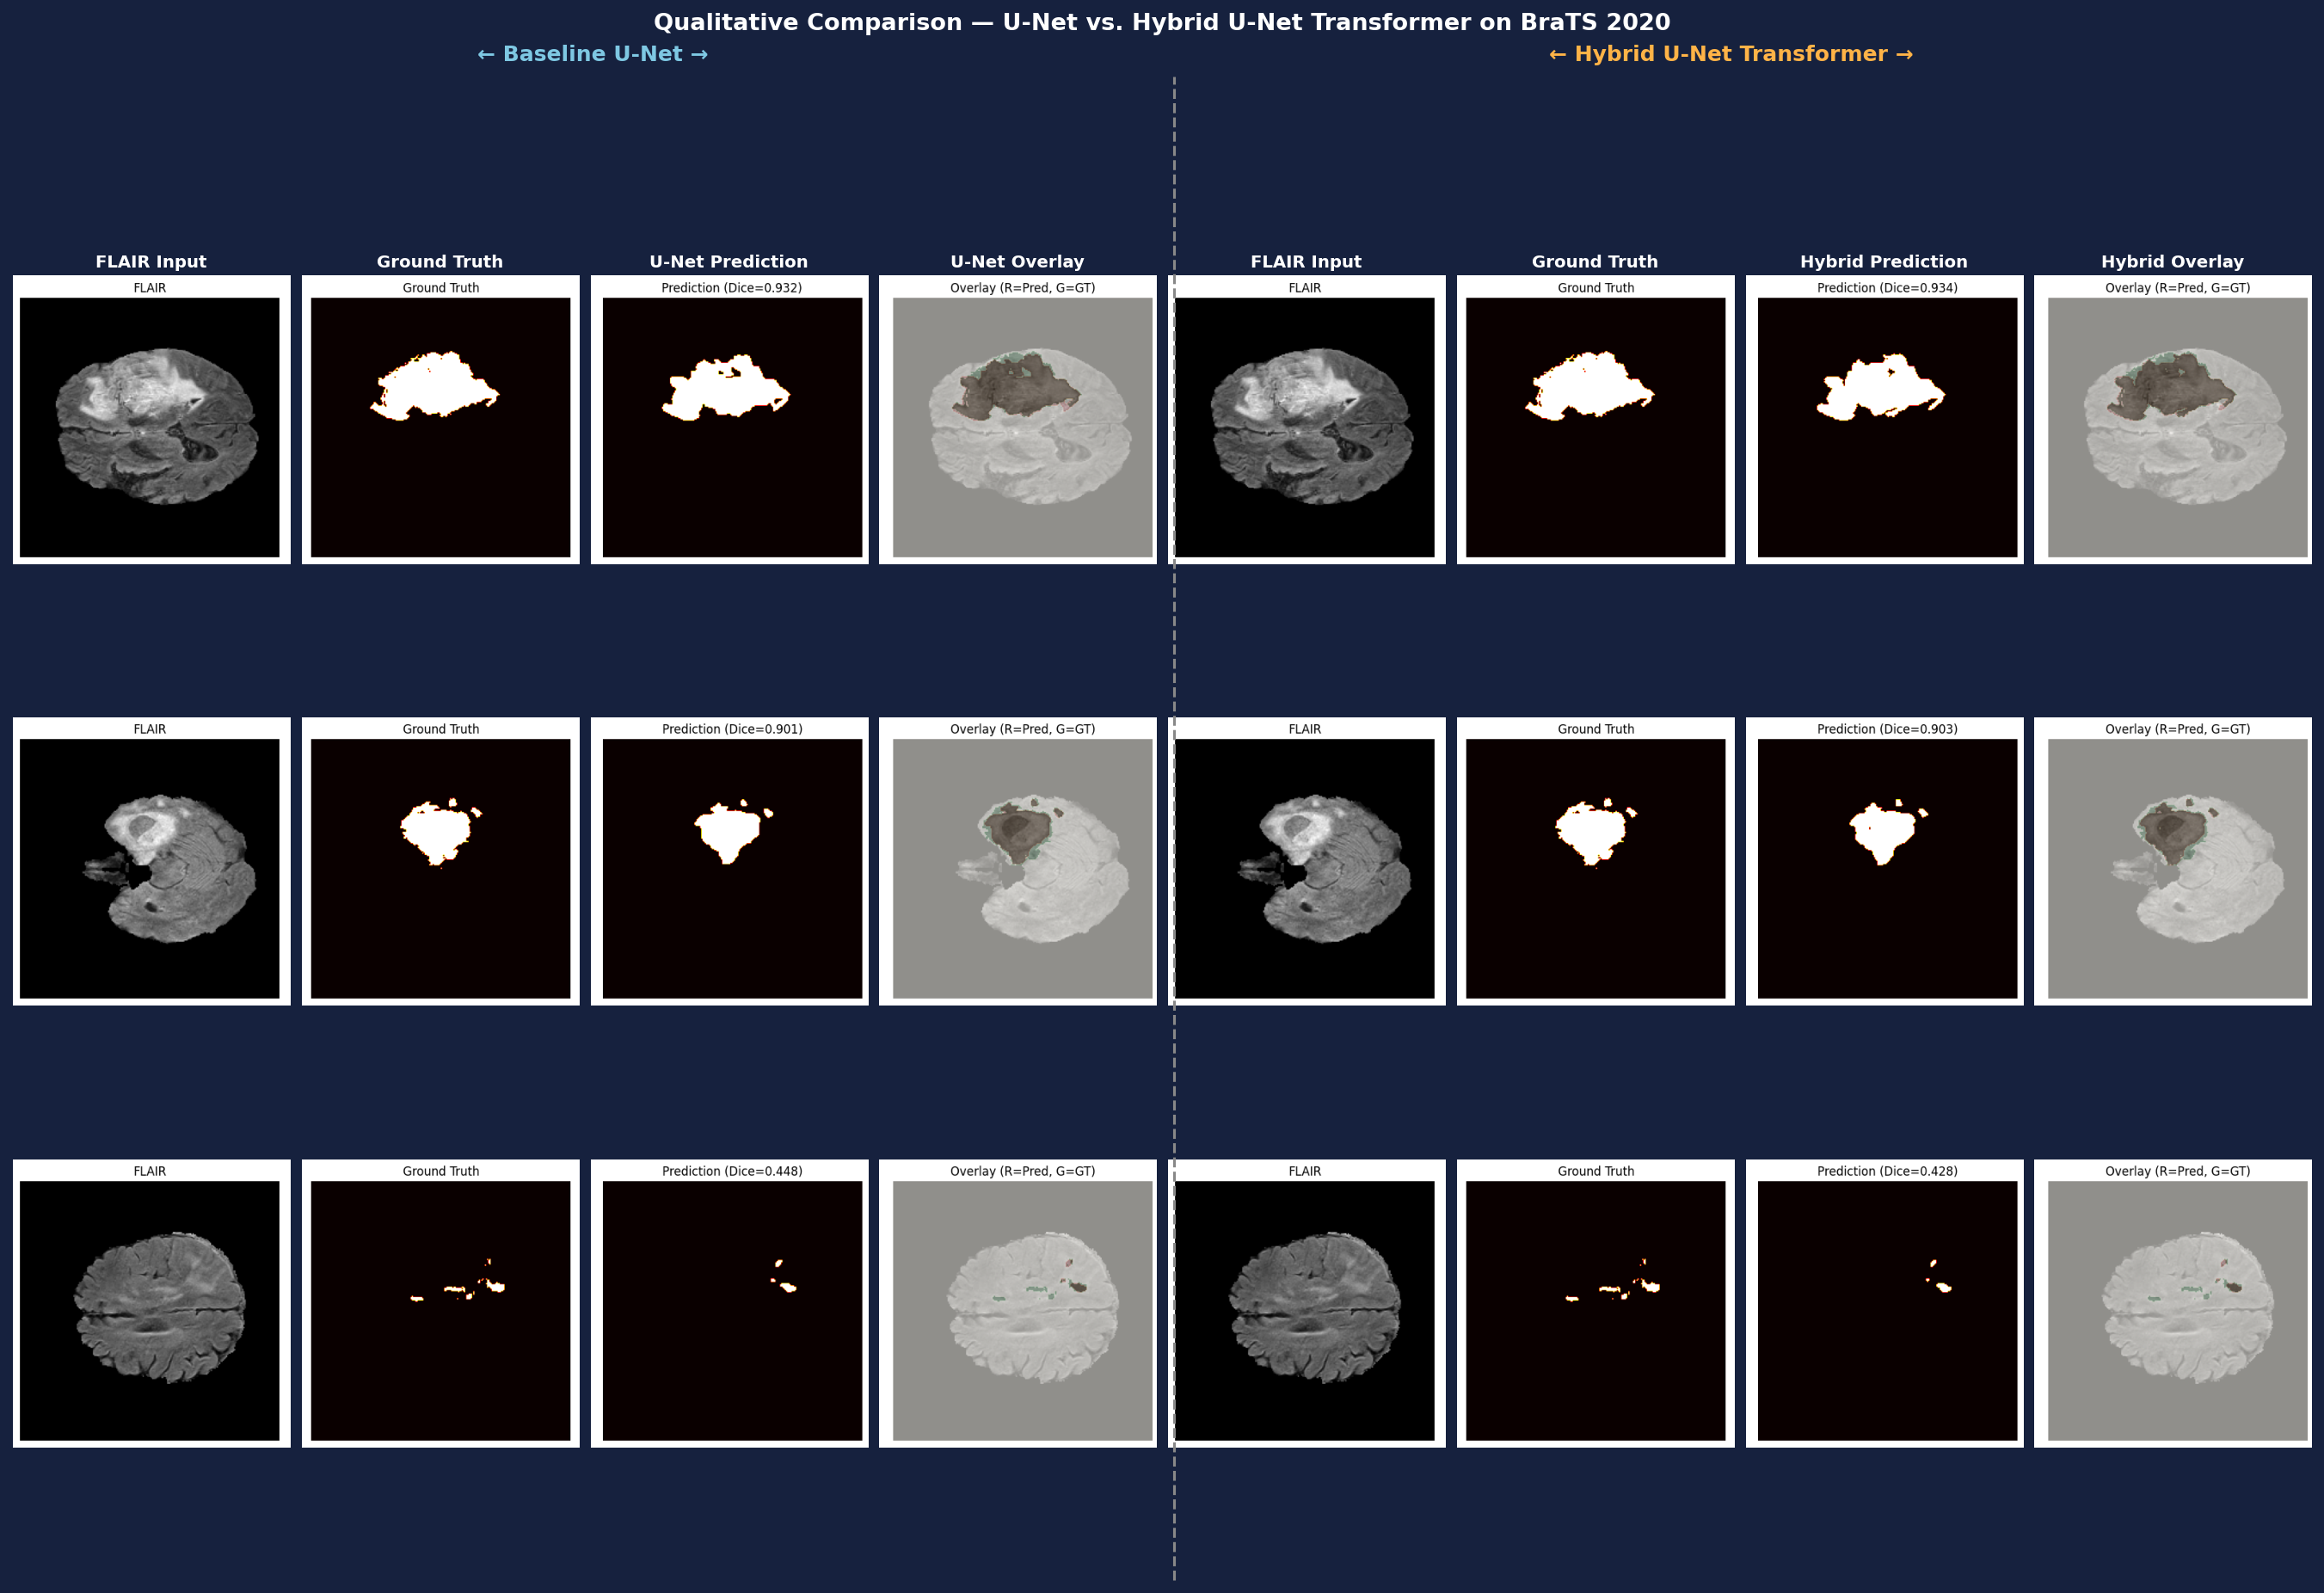
\includegraphics[width=0.98\textwidth]{fig4_qualitative.png}
  \captionof{figure}{Qualitative comparison on three BraTS~2020 validation cases.
  \textit{Left four columns:} Baseline U-Net. \textit{Right four columns:} Hybrid
  U-Net Transformer. Each group shows FLAIR input, ground truth mask, model prediction,
  and overlay (red\,=\,prediction, green\,=\,GT). The Hybrid model produces
  smoother boundaries and fewer false-positive fragments in challenging cases (rows~2--3).}
  \label{fig:qual}
\end{center}

\end{document}
